\documentclass[conference]{IEEEtran}
\IEEEoverridecommandlockouts
% The preceding line is only needed to identify funding in the first footnote. If that is unneeded, please comment it out.
\usepackage{cite}
\usepackage[fleqn]{amsmath}
\usepackage{amssymb,amsfonts}
\usepackage{algorithmic}
\usepackage{graphicx}
\usepackage{textcomp}
\usepackage{xcolor}
\usepackage{balance}
\usepackage{algorithm}
\usepackage[utf8]{inputenc}
\usepackage{arevmath} 
\def\BibTeX{{\rm B\kern-.05em{\sc i\kern-.025em b}\kern-.08em
    T\kern-.1667em\lower.7ex\hbox{E}\kern-.125emX}}

\makeatletter
\newcommand{\linebreakand}{%
  \end{@IEEEauthorhalign}
  \hfill\mbox{}\par
  \mbox{}\hfill\begin{@IEEEauthorhalign}
}
\makeatother


\begin{document}

\title{Drug Target protein interaction prediction by PSSM and LOOP method with extra Ligand based features\\}

\author{\IEEEauthorblockN{C.Vijayabaskar(2017103048)}
\IEEEauthorblockA{\textit{Dept. of Computer science} \\
\textit{Anna University}\\
Chennai }
\and
\IEEEauthorblockN{V.Rohith(2017103580)}
\IEEEauthorblockA{\textit{Dept. of Computer science} \\
\textit{Anna University}\\
Chennai }
\and
\IEEEauthorblockN{K.Sathish Kumar(2017103588)}
\IEEEauthorblockA{\textit{Dept. of Computer science} \\
\textit{Anna University}\\
Chennai }
\linebreakand
\IEEEauthorblockN{Guided by}
\IEEEauthorblockN{G.Sudhakaran}
\IEEEauthorblockA{\textit{Dept. of Computer science} \\
\textit{Anna University}\\
Chennai }
}

\maketitle

\begin{abstract}
Predicting the target-drug interactions (DITs) is of great important for screening new drug candidate and understanding biological processes. However, identifying the drug-target interactions through traditional experiments is still costly, laborious and complicated. Thus, there is a great need for developing reliable computational methods to effectively predict DTIs. In this study, a novel computational method combining local optimal oriented pattern LOOP), Position Specific Scoring Matrix (PSSM) and Rotation Forest (RF) for predicting DTI. Specifically, the target protein sequence is firstly transformed as the PSSM, in which the evolutionary information of protein is retained. Then, the LOOP is used to extract the feature vectors from PSSM, and the sub-structure information of drug molecule is represented as fingerprint features. And the ligand based features of drug and target is appended to the feature set. Finally, Rotation Forest classifier is adopted to infer the potential drug-target interactions. When experiment is carried out with drugbank dataset the proposed system performs well with an accuracy of 89.3\%. The comprehensive experimental results illustrate that the proposed method is reliable and efficiency for predicting DTIs.
\end{abstract}

\begin{IEEEkeywords}
PSSM; LOOP; Molecular fingerprint; PSI-BLAST; Rotation forest
\end{IEEEkeywords}

\section{Background}
Drug target interaction is a prominent research area in the field of drug discovery. It refers to the recognition of interactions between chemical compounds and the protein targets. Wet lab experiments to identify these interactions are expensive as well as time consuming. Drug-Target Interaction Prediction (DTI) is an important application of machine learning in medicine industry, the importance is coming from the fact of saving the time and cost of the drugs development.Large numbers of DTIs have been uncovered in databases such as DrugBank, Matador, and CTD, but many DTIs remain to be discovered. These public databases store a number of known drug-target interactions which validate through experimental.

Drug is a chemical substance, typically of known structure, which, when administered to a living organism, produces a biological effect. A pharmaceutical drug, also called a medication or medicine, is a chemical substance used to treat, cure, prevent, or diagnose a disease or to promote well-being. The most widely used drugs in the world include caffeine, nicotine and alcohol, etc. Target proteins are functional biomolecules that are addressed and controlled by biologically active compounds. They are used in the processes of transduction, transformation and conjugation. They are used by the body to build and repair the body e.g. enzymes which are used to speed up chemical reactions such as insulin or antibodies which are used to fight off foreign particles in the body such as viruses. Proteins are made up of chained combinations of amino acids and do not have a fixed length, the amino acids come from the amino acid alphabet of length 20 but proteins can have any length. 

Computational methods for DTI prediction are divided into 3 main approaches:
\begin{itemize}
\item Ligand based
\item Docking simulation
\item Chemogenomic
\end{itemize}

Ligand based approaches are built upon the concept that similar molecules have similar properties and therefore should bind to the same group of proteins. Docking Simulation approaches are used for structure based drug design, where the interaction between a protein and a drug is simulated and scored, according to the intermolecular interaction energy, using 3D structures. Chemogenomic approaches are based on the chemical space of compounds, genomic space of target proteins and/or the pharmacological space (interactions between proteins and drugs) to predict new potential interactions.Modern technologies have mitigated the problem, leveraging the development of new drugs. However, drug development remains extremely expensive and time consuming. Many machine learning approaches have been proposed over the years for DTI prediction. Nevertheless, prediction accuracy and efficiency are persisting problems that still need to be tackled. Here, proposed a new learning method which addresses DTI prediction which uses chemogenomic way of predicting.

\section{Related works}
Chemogenomics, an emerging research area focused on the systematic examination of the biological impact of a broad series of minute molecular-weighting ligands on a broad raiment of macromolecular target spots. Additionally, with the advancement in time, the complexity of the algorithms is increasing which may result in the entry of big data technologies. It integrates target and drug discovery by using active compounds, which function as ligands, as probes to characterize proteome functions. The interaction between a small compound and a protein induces a phenotype. Nidhi \cite{b9} describes the Prediction of Biological Targets for Compounds Using Multiple-Category Bayesian Models Trained on Chemogenomics Databases. It is useful for improving knowledge in chemogenomics databases and for predicting new targets for orphan compounds.

In order to improve the drug discovery efficiency, there is a great need for the development of accurate computational approaches that can predict potential drug-target interactions to direct the experimental verification. Y. Liu \cite{b17} propose a novel drug-target interaction prediction algorithm, namely neighborhood regularized logistic matrix factorization (NRLMF). Specifically the proposed NRLMF method focuses on modeling the probability that a drug would interact with a target by logistic matrix factorization, where the properties of drugs and targets are represented by drug-specific and target-specific latent vectors, respectively.  The drawback is that lack of couple logistic matrix factorization with the multiple kernel learning techniques leads to low accuracy. W. Zhang \cite{b13} describes the drug-drug interaction prediction as a matrix completion task, and project drugs in the interaction space into a low-dimensional space. By considering the drug features, i.e., substructures, targets, enzymes, transporters, pathways, indications, side effects, and off side effects, to calculate drug-drug similarities, and assume them as manifolds in feature spaces. MRMF is promising and effective for the prediction of drug-drug interactions. But there defines no accurate methods on how to combine diverse features in a manifold regulation.

The neighbor molecules plays a huge role in the interaction between thee drug and the target. J.P. Mei \cite{b3} present a simple procedure called neighbor-based interaction-profile inferring (NII) and integrate it into the existing BLM method to handle the new candidate problem. Specifically, the inferred interaction profile is treated as label information and is used for model learning of new candidates. This demonstrates the effectiveness of the NII strategy and also shows the great potential of BLM–NII for prediction of compound–protein interactions. But there is a deterioration in the prediction performance and limited exploration in local and global information in model learning. The development of computational methods for drug-target interaction prediction is an urgent task of theoretical interest and practical significance. W.Zhang \cite{b14} propose a label propagation method with linear neighborhood information (LPLNI) for predicting unobserved drug-target interactions. It calculates drug-drug linear neighborhood similarity in the feature spaces, by considering how to reconstruct data points from neighbors. This experiment doesn’t show how to utilize the unknown data for drug-target interaction.

Semi-supervised learning is an approach to machine learning that combines a small amount of labeled data with a large amount of unlabeled data during training. Semi-supervised learning falls between unsupervised learning (with no labeled training data) and supervised learning (with only labeled training data). It is a special instance of weak supervision. H. Chen \cite{b1} proposed a semi-supervised learning method NetCBP to address this problem by using labeled and unlabeled interaction information. Assuming coherent interactions between the drugs ranked by their relevance to a query drug, and the target proteins ranked by their relevance to the hidden target proteins of the query drug, a learning framework maximizing the rank coherence with respect to the known drug-target interactions. It focuses on improving detection of drug-target interactions by integrating the drug similarity network and the target similarity network to better summarize sparse interactions for a global comparison of all possible drug-target interactions.

As discussed earlier the matrix formatted feature extraction caries more information and it is computationally powerful and more accurate. L. Wang \cite{b5} describes a novel computational model is developed for predicting potential drug-target interactions under the theory that each drug-target interaction pair can be represented by the structural properties from drugs and evolutionary information derived from proteins. Specifically, the protein sequences are encoded as Position-Specific Scoring Matrix (PSSM) descriptor which contains information of biological evolutionary and the drug molecules are encoded as fingerprint feature vector which represents the existence of certain functional groups or fragments. PSSM is matrix formatted features which carries the information of the protein sequence. This is similar to a substitution score matrix, but instead of specifying the scores or distances for amino acid or nucleotide replacements, a PSSM specifies the scores for observing particular amino acids or nucleotides at specific positions.

Rotation Forest is a recently proposed method for building classifier ensembles using independently trained decision trees. It was found to be more accurate than bagging, AdaBoost and Random Forest ensembles across a collection of benchmark data sets. Silico methods are urgently needed to predict drug-target interactions in a genome-wide manner. In \cite{b16}, they design a new in silico approach, named DTIRF, to predict the DTI combine feature weighted Rotation Forest (FwRF) classifier with protein amino acids information. More specifically, Position-Specific Score Matrix (PSSM) is used to numerically convert protein sequences and utilize Pseudo Position-Specific Score Matrix (PsePSSM) to extract their features. Then a unified digital descriptor is formed by combining molecular fingerprints representing drug information. Finally, the feature weighted rotation forest is applied to data sets.

From the works it is clear that identifying drug-target interactions (DTIs) is a major challenge in drug development. Traditionally, similarity-based approach is used to predict DTI. This method use drug and target similarity matrices to infer the potential drug-target interactions. But these techniques do not handle biochemical data directly. Hence in the proposed system we use PSSM matrices in order to carry at most information to the feature set. And the inclusion of structure based information further improve the prediction to an extent. Data incompleteness is the major issue for such prediction problem. Since it is related to drugs and chemical compounds the complete data is hard to achieve. Many sources have data with incomplete information. Chemical compound react to one another based on many properties. Since it is not easy to carry all the physical and chemical properties in the training process the accuracy of the prediction is low. The necessity of physical and chemical property is handles by the ligand features in the proposed system.

\section{Proposed System}
The proposed system introduces a novel computational method based on target protein sequence and drug substructure fingerprints is proposed. It uses the Chemogenomic approach of predicting the interaction. The method combines local optimal oriented pattern (LOOP), position specific scoring matrix (PSSM) and rotation forest (RF) for predicting DTIs. Specially, the target protein sequence is first transformed into PSSM in order to retain biological evolutionary information, and consider molecular substructure fingerprints are considered as the feature of drugs. Then local optimal oriented pattern (LOOP) is applied to extract the 256 feature vectors from PSSM. Ligand based features are taken into consideration for feature set. Finally, rotation forest classifier is applied to predict the DTIs.

\begin{figure}[htbp]
\centerline{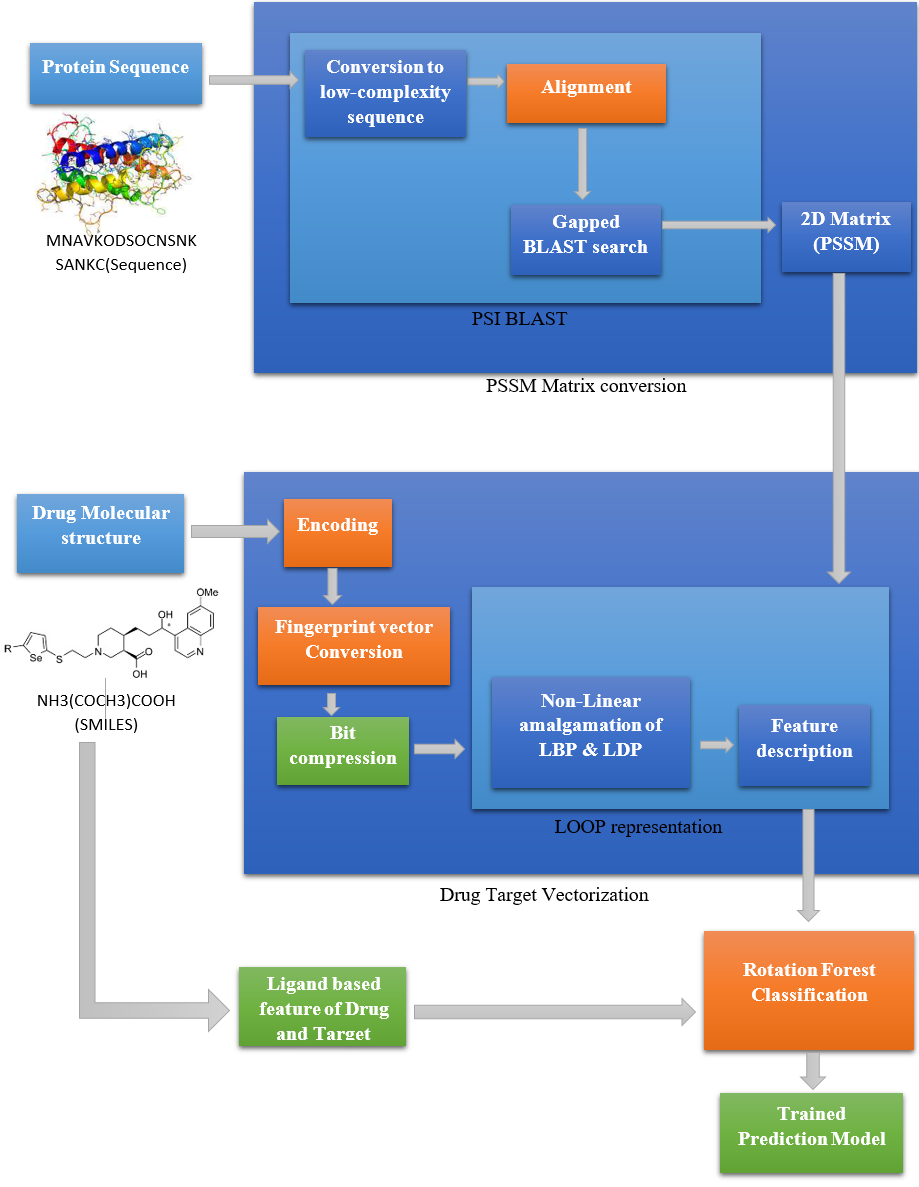
\includegraphics[scale=0.34]{figures/fig1.png}}
\caption{Complete Architecture diagram}
\label{f1}
\end{figure}

The overall architecture diagram for the proposed system is shown in figure.\ref{f1}. The proposed work is split into four major phases namely fingerprint vectorization, PSSM generation, LOOP formation and Rotation forest classifier. The final result is the trained model for predicting the drug - target interaction. On drug side, the fingerprint vectorization includes the extraction of morgan fingerprint from the drug SMILES. It comprises of encoding the SMILES into Morgan fingerprint followed by the bit compression of the generated fingerprint. On the other hand, the target sequence is first converted into PSSM with PSI-BLAST, which includes the conversion of protein sequence into low complexity sequence followed by alignment and gapped blast search. The generated PSSM is converted into LOOP, which incorporates the neighboring compound features. In addition to the drug structural features, the ligand based features of the drug is added to the existing features. Finally, Rotation forest classifier algorithm is applied on the drug and target features. With some hyper parameter tuning the algorithm is tuned to exhibit in an efficient manner. At last, a trained model which can be used for predicting the drug – target interaction is obtained.



\subsection{Fingerprint vectorization}

Molecular fingerprints are essential cheminformatics tools for virtual screening and mapping chemical space. Among the different types of fingerprints, substructure fingerprints perform best for small molecules such as drugs, while atom-pair fingerprints are preferable for large molecules such as peptides \cite{b18}. Molecular fingerprints are a way to represent molecules as mathematical objects. One of the most common molecular fingerprinting methods is Extended Connectivity Finger Printing (ECFP). This family of fingerprints, also known as circular fingerprints, is built by applying the Morgan algorithm to a set of user-supplied atom invariants. When generating Morgan fingerprints, the radius of the fingerprint must also be provided. The figure.\ref{f2} represents the flow of the generation of compressed finger print. The process involves the assignment of each atom with identifier followed by updating and removing duplicates. Finally wrapping up into 2048 byte vector. It is then compressed into 256 bytes. The input for fingerprint vectorization is SMILES. eg. N[C@@H](CC(O)=O)C(O)=O. The output is the 256 byte vector.

\begin{figure}[htbp]
\centerline{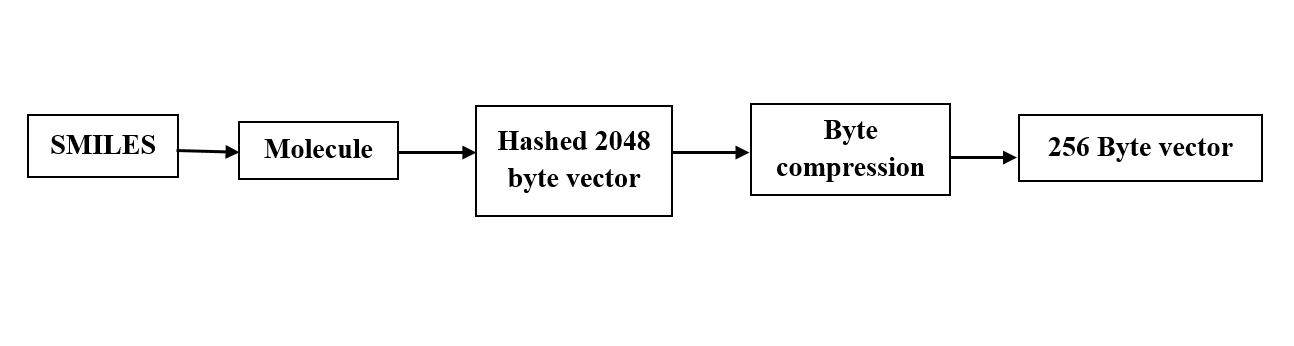
\includegraphics[scale=0.27]{figures/fig2.png}}
\caption{Flow of fingerprint vector generation}
\label{f2}
\end{figure}


\subsection{PSSM generation}
A PSSM, or Position-Specific Scoring Matrix, is a type of scoring matrix used in protein BLAST searches in which amino acid substitution scores are given separately for each position in a protein multiple sequence alignment. Thus, a Tyr-Trp substitution at position A of an alignment may receive a very different score than the same substitution at position B. This is in contrast to position-independent matrices such as the PAM and BLOSUM matrices, in which the Tyr-Trp substitution receives the same score no matter at what position it occurs. PSSM scores are generally shown as positive or negative integers \cite{b7}. Positive scores indicate that the given amino acid substitution occurs more frequently in the alignment than expected by chance, while negative scores indicate that the substitution occurs less frequently than expected. PSSMs can be created using PSI-BLAST, which finds similar protein sequences to a query sequence, and then constructs a PSSM from the resulting alignment. Alternatively, PSSMs can be retrieved from the NCBI CDD database, since each CD is represented by a PSSM that encodes the observed substitutions in the seed alignments. PSI-BLAST (Position-Specific Iterative Basic Local Alignment Search Tool) derives a position-specific scoring matrix (PSSM) or profile from the multiple sequence alignment of sequences detected above a given score threshold using protein–protein BLAST. This PSSM is used to further search the database for new matches, and is updated for subsequent iterations with these newly detected sequences \cite{b10}. The figure.\ref{f3} represents the flow of PSSM generation from the protein sequence, where protein sequence undergoes subsequent steps of PSI-BLAST to generate PSSM.
 
\begin{figure}[htbp]
\centerline{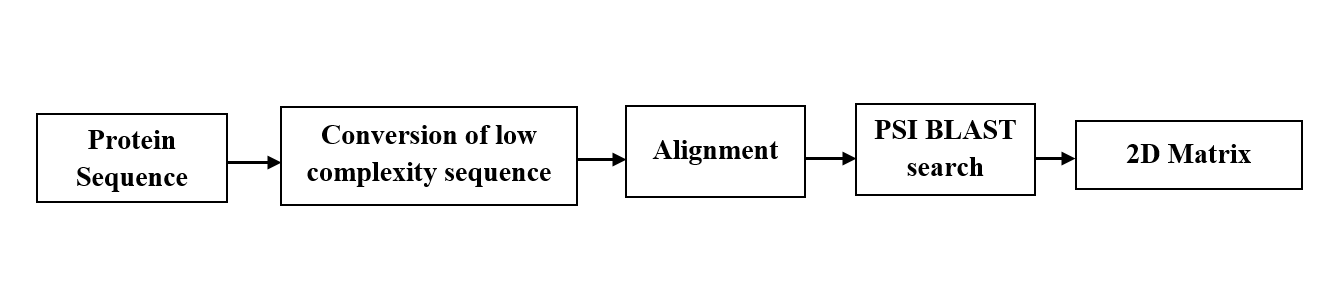
\includegraphics[scale=0.27]{figures/fig3.png}}
\caption{Flow of PSSM generation}
\label{f3}
\end{figure}

The input is the FASTA file of the individual proteins. It is blast against the Nr database. The output is an ascii formatted PSSM file.

\subsection{LOOP formation}
The LOOP binary descriptor (local optimal-oriented pattern) that encodes rotation invariance into the main formulation itself. This makes any post processing stage for rotation invariance redundant and improves on both accuracy and time complexity \cite{b11}\cite{b12}. LBP is a popular descriptor which captures the local intensity variation patterns of an image and has good discrimination characteristics. Let $i_c$ be the intensity of an image I at pixel ($x_c$ , $y_c$ ) and in (n = 0,..., 7) be the intensity of a pixel in the 3 × 3 neighborhood of ($x_c$ , $y_c$ ) excluding the center pixel ic . Then the LBP value for the pixel ($x_c$ , $y_c$ ) is given by

\begin{equation}
\label{eq1}
LBP (x_c , y_c ) = \sum\limits_{n=0}^{7} S(i_n - i_c).2^{n}
\end{equation}

where

\[ s(x) =
  \begin{cases}
    1       & \quad \text{if } n>=0\\
    0  & \quad \text{otherwise}
  \end{cases}
\]

A major disadvantage of LBP is the arbitrary sequence of binarization weights. Depending on the chosen starting pixel of the sequence of binary weights (2n , n = 0,..., 7), the eight neighbors of the output 3 × 3 grid are allocated subsequent weightage n sequentially. LDP is an improved local pattern descriptor which incorporates a directional component by using Kirsch compass kernels. It was shown to be less susceptible to noise than the traditional LBP operator. Let $i_c$ be the intensity of an image I at pixel ($x_c$ , $y_c$ ) and in , n = 0, 1,..., 7 be the intensity of a pixel in the 3 × 3 neighborhood of ($x_c$ , $y_c$ ) excluding the center pixel $i_c$ . 3 × 3 Kirsch edge detectors centered at ($x_c$ , $y_c$ ) in eight possible directions are given in figure.\ref{f4}. The eight responses of the Kirsch masks are mn , n = 0,..., 7 corresponding to pixels with intensity in , n = 0,..., 7 and let mk be the kth highest Kirsch activation. Then the LDP value for the pixel (xc , yc ) is given by

\begin{equation}
\label{eq2}
LDP_k (x_c , y_c ) = \sum\limits_{n=0}^{7} S(m_n - m_k).2^{n}
\end{equation}

where

\[ s(x) =
  \begin{cases}
    1       & \quad \text{if } n>=0w\\
    0  & \quad \text{otherwise}
  \end{cases}
\]

\begin{figure}[htbp]
\centerline{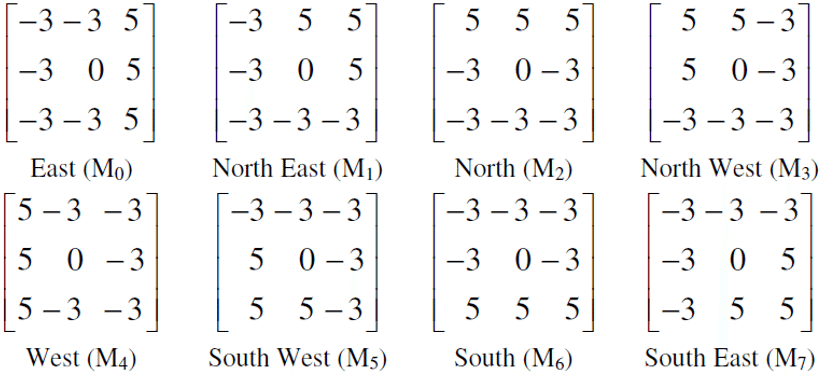
\includegraphics[scale=0.27]{figures/fig4.png}}
\caption{KIRSCH masks}
\label{f4}
\end{figure}


The major disadvantage of LBP and LDP is the arbitrary sequence of binarization weights that adds dependency to orientation. LDP also suffers from the empirical assignment of value to the threshold variable, which puts an ad hoc restriction on the number of bits allowed to be 1, thus reducing the number of possible words, as discussed before. LOOP presents a nonlinear amalgamation of LBP and LDP that overcomes these drawbacks while preserving the strengths of each. Let $i_c$ be the intensity of an image I at pixel ($x_c$ , $y_c$ ) and in (n = 0, 1,..., 7) be the intensity of a pixel in the 3 × 3 neighborhood of ($x_c$ , $y_c$ ) excluding the center pixel $i_c$ . The eight Kirsch masks, as used in LDP previously, are oriented in the direction of these eight neighboring pixels in (n = 0, 1,..., 7), thus giving a measure of the strength of intensity variation in those directions, respectively. Then the LOOP value for the pixel (xc , yc ) is given by

\begin{equation}
\label{eq3}
LOOP (x_c , y_c ) = \sum\limits_{n=0}^{7} S(i_n - i_c).2^{w_{n}}
\end{equation}

where

\[ s(x) =
  \begin{cases}
    1       & \quad \text{if } n>=0\\
    0  & \quad \text{otherwise}
  \end{cases}
\]

Thus, the LOOP descriptor encodes rotation invariance into the main formulation. Moreover, the proposed LOOP algorithm also negates the empirical assignment of the value of the parameter k in the traditional LDP method. The output is the 256 feature vector.

\subsection{Ligand based features}
Ligand-based drug design (or indirect drug design) relies on knowledge of other molecules that bind to the biological target of interest. These other molecules may be used to derive a pharmacophore model that defines the minimum necessary structural characteristics a molecule must possess in order to bind to the target. In other words, a model of the biological target may be built based on the knowledge of what binds to it, and this model in turn may be used to design new molecular entities that interact with the target.

On drug side 96 feature descriptors are taken into consideration which includes, Number of hydrogen donors, acceptors, number of ring count, solubility value, melting and boiling point etc. Rdkit is an open source library which gives information about the drugs. With the help of rdkit the extraction of necessary drug descriptors information is made easier.

On target side the CTD (Composition – Transition -Distribution) information are extracted. Dubchak et al. (1995) introduced the concept of CTD feature while making the prediction for different classes of protein folding. Since its introduction, the CTD feature has been successfully employed in many functional and structural related studies of proteins (Govindan and Nair, 2011). In CTD, C (composition) stands for the compositions of amino acids, T (transition) represents the percentage with which frequency of amino acids with specific properties is followed by amino acids with other properties and D (distribution) determines the length of the sequence within which the 1st as well as 25, 50, and 75 percent’s of amino acids of certain characteristics are located.

\subsection{Rotation forest }
Rotation Forest is a recently proposed method for building classifier ensembles using independently trained decision trees \cite{b4}. It was found to be more accurate than bagging, AdaBoost and Random Forest ensembles across a collection of benchmark data sets. In rotation forest the training data for a base classifier, the feature set is randomly split into K subsets (K is a parameter of the algorithm) and principal component analysis (PCA) is applied to each subset. All principal components are retained in order to preserve the variability information in the data. Thus, K axis rotations take place to form the new features for a base classifier. The idea of the rotation approach is to encourage simultaneously individual accuracy and diversity within the ensemble. Diversity is promoted through the feature extraction for each base classifier. Decision trees were chosen here because they are sensitive to rotation of the feature axes, hence the name "forest". Accuracy is sought by keeping all principal components and also using the whole data set to train each base classifier.


\section{Experimental setup}

\subsection{Dataset and hyper parameters}
In this study, the structural information of the drugs and the sequence information of the targets are considered as the primary dataset. These datasets are collected from DrugBank, KEGG BRITE, SuperTarget \& Matador, and BRENDA which were considered as high-reliability databases \cite{b15}. In the proposed system, among 11150 drug samples drugs that are approved by the NCBI are used. And among 5257 target samples, targets that found in human being are utilized. In this study we targeted the approved drugs and human targets as reported in table.\ref{tab1}.

The parameters for PSI-Blast query need to be optimized. Here we took the number of iterations as 3 with inclusion ethresh value of 0.001. Especially in rotation forest algorithm, optimizing two corresponding parameters of K and L for capturing best performance of parameters is necessary in the prediction model \cite{b20}. Where K is the number of feature subsets and L represents the number of decision tree. The grid research method tries different combination of the parameters as input and selects the optimized parameters K and L. The optimal parameters K=26 and L=25 have better performance than other parameter. In addition to this parameter some other parameters are also optimized like bootstrap=True, criterion=gini and maxfeatures=None. 

\subsection{Evaluation metrics}
In this work, in order to evaluate the performance of the proposed method, the evaluation measures such as the overall prediction accuracy, precision, sensitivity (recall), f-score, cross validation and ROC is used.

\begin{equation}
\label{eq4}
Accuracy = \frac{\text{TP + TN}}{\text{TP + TN + FP + FN} }
\end{equation}

\begin{equation}
\label{eq5}
Precision = \frac{\text{TP}}{\text{TP + FP} }
\end{equation}

\begin{equation}
\label{eq6}
Recall = \frac{\text{TP}}{\text{TP + FN} }
\end{equation}

\begin{equation}
\label{eq7}
f1 score = 2. \frac{\text{(Precision . Recall)}}{\text{(Precision + Recall)} }
\end{equation}

Here, the false positive (FP) is the number of drug-target pairs which are predicted as interacting pairs incorrectly; true negative (TN) denotes the count of samples which are classified as non-interacting correctly; true positive (TP) represents the number of samples which are predicted as interacting pairs correctly and false negative (FN) is the number of true samples which are predicted as non-interacting pairs incorrectly.Moreover, the receiver operating characteristic (ROC) curves were also computed to evaluate the performance of the proposed method. To Summarize the ROC curve in a numerical way, the area under an ROC curve (AUC) was also computed for better analyze the propose method.

\begin{table}[htbp]
\caption{Dataset information}
\begin{center}
\begin{tabular}{|c|c|}
\hline
\textbf{Total Drugs}&\textbf{Total Targets} \\
\hline
11834 & 5260 \\
\hline
\textbf{Filtered Drugs}&\textbf{Filtered Targets} \\
\hline
11150 & 5257 \\
\hline
\textbf{Approved Drugs}&\textbf{Human Targets} \\
\hline
2500 & 2882 \\
\hline
\multicolumn{2}{|c|}{\textbf{Total Interactions}} \\
\hline
\multicolumn{2}{|c|}{26840}\\
\hline
\end{tabular}
\label{tab1}
\end{center}
\end{table}

\section{Resullt and Discussion}

\subsection{Comparisionn with varients of proposed system}
The evaluation of the proposed system was experimented in the drugbank dataset. The evaluation is carried under two phases: Without the inclusion of the ligand based features and with the inclusion of the ligand based features in the feature set. From table. \ref{tab2} it is clearly seen that the addition of ligand features improve the model to a considerable extent. Accuracy got improved from 86.7\% to 89.3\%. Likewise precision and recall got improved from 86.6\% to 90.6\% and 70.8\% to 75.4\% respectively. Figure.\ref{} reports the ROC curve of the model with and without ligand features with an AUC improvement from 0.919 to 0.938.

\begin{table}[htbp]
\caption{Metric scores of model with and without ligand based features}
\begin{center}
\begin{tabular}{|c|c|c|}
\hline
&\textbf{Without Ligand}&\textbf{With Ligand} \\
&\textbf{based Features}&\textbf{based Features} \\
\hline
\textbf{Accuracy}&0.8679 & 0.8934 \\
\hline
\textbf{Precision}&0.8667 & 0.9064 \\
\hline
\textbf{Recall}& 0.7086 & 0.7549 \\
\hline
\textbf{f1-scorel}&0.7797 & 0.8237 \\
\hline
\textbf{Mean error rate}& 0.1321 & 0.1066 \\
\hline
\end{tabular}
\label{tab2}
\end{center}
\end{table}

\begin{figure}[htbp]
\centerline{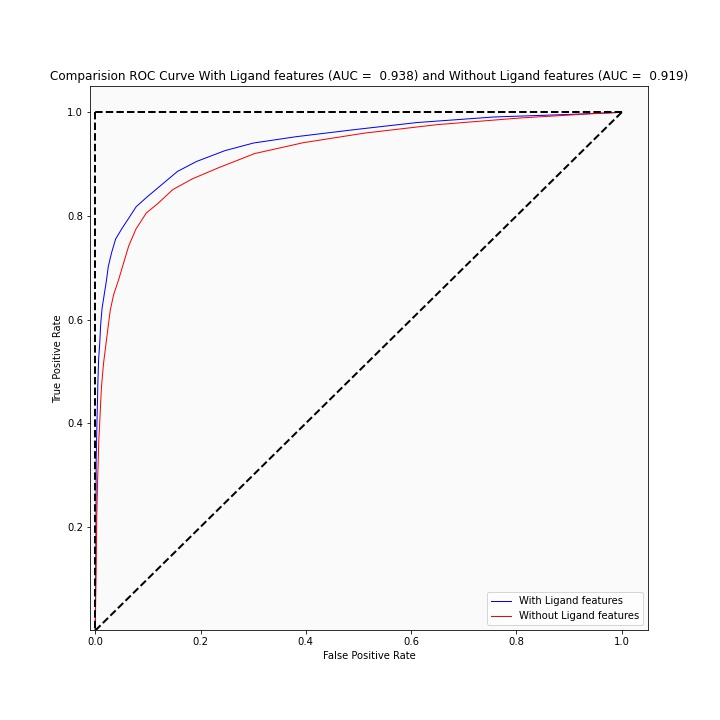
\includegraphics[scale=0.27]{figures/fig5.jpeg}}
\caption{ROC Curve for model with and without ligand based features}
\label{f5}
\end{figure}
\subsection{Comparisionn with existing systems}
Nowadays, a lot of computational methods have been proposed for predicting protein-protein interactions. In this work, we compared the prediction performance between our proposed method and the existing methods including bipartite graph learning \cite{b19}, deep learning \cite{b8}, SIMCOMP \cite{b2} and KBMF2K \cite{b6}. Table.\ref{tab3} represents the AUC score of the previous drug-target prediction works. It can be observed that the proposed method has a significant improvement in prediction performance.

\begin{table}[htbp]
\caption{Metric scores of model with and without ligand based features}
\begin{center}
\begin{tabular}{|c|c|}
\hline
\textbf{Previous models/ methods}&\textbf{Area under curve (AUC)} \\
\hline
Bipartite graph learning&0.904 \\
\hline
Deep learning&0.915 \\
\hline
SIMCOMP& 0.863 \\
\hline
KBMF2K&0.832 \\
\hline
\textbf{Our Proposed system}& 0.938 \\
\hline
\end{tabular}
\label{tab3}
\end{center}
\end{table}
\begin{figure}[htbp]
\centerline{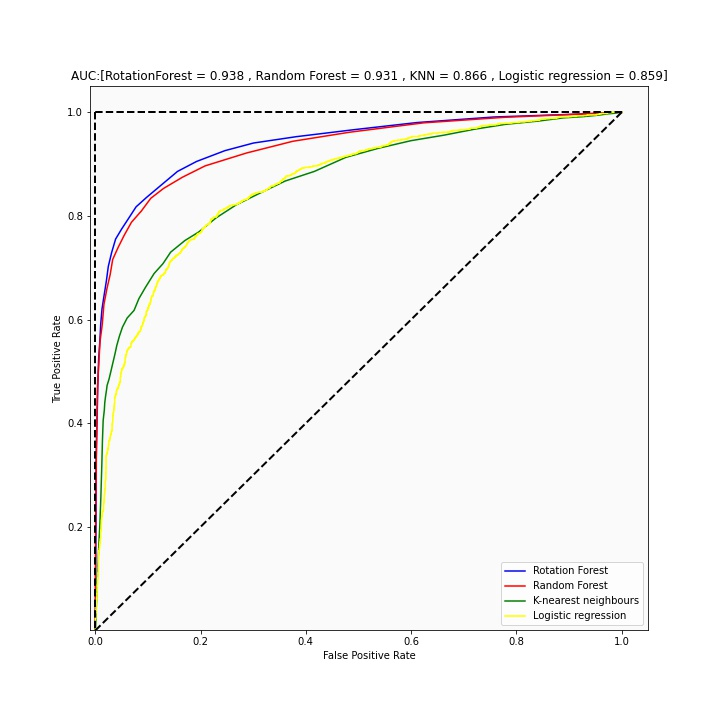
\includegraphics[scale=0.27]{figures/fig6.jpeg}}
\caption{ROC of different models}
\label{f6}
\end{figure}
On comparison with other machine learning models, it is clearly seen that the proposed system is performing quiet well in all aspects which is proved by the ROC curve of different models as in figure.\ref{f6}. It is better in accuracy, precision and recall scores against random forest and K- nearest neighbors.
\section{Conclusion and future works}
Here, proposed a novel computational approach combines local optimal oriented pattern (LOOP), position specific scoring matrix (PSSM), ligand based features of drug and target, and rotation forest (RF) classifier. The proposed method for predicting DTIs is by fusing molecular fingerprint information and protein sequence information. In the experiment, tenfold cross-validation method for further evaluating the potential drug-target interaction on drugbank datasets, including approved drugs and human proteins is applied. The proposed method achieved an average accuracy of 89.3\%. According to comprehensive experimentation, the predictive performance of proposed method was significantly well in predicting DTIs, especially when comparing different classifier, the proposed method shows the robust and stable in predicting DTIs. The main improvement come from the addition of ligand based feature to the existing feature set. And also the feature extraction of LOOP which integrates the strength of two texture descriptors local binary pattern (LBP) and local directional pattern (LDP) and find the texture intensity differences in drug-target pairs. However, due to the limitation of the feature extraction method, still there is a need to make great efforts to improve the effectiveness of feature extraction methods.

\begin{thebibliography}{00}
\bibitem{b1}H. Chen and Z. Zhang, "A semi-supervised method for drug-target interaction prediction with consistency in networks", PLoS ONE, vol. 8, no. 5, May 2013.
\bibitem{b2}H. Öztürk, E. Ozkirimli and A. Özgür, "A comparative study of SMILES-based compound similarity functions for drug-target interaction prediction", BMC Bioinf., vol. 17, no. 1, pp. 128, Mar. 2016.
\bibitem{b3} J.-P. Mei, C.-K. Kwoh, P. Yang, X.-L. Li and J. Zheng, "Drug–target interaction prediction by learning from local information and neighbors", Bioinformatics, vol. 29, no. 2, pp. 238-245, Jan. 2013.
\bibitem{b4} J. J. Rodriguez, L. I. Kuncheva and C. J. Alonso, "Rotation forest: A new classifier ensemble method", IEEE Trans. Pattern Anal. Mach. Intell., vol. 28, no. 10, pp. 1619-1630, Aug. 2006.
\bibitem{b5}L. Wang, Z.-H. You, X. Chen, X. Yan, G. Liu and W. Zhang, "RFDT: A rotation forest-based predictor for predicting drug-target interactions using drug structure and protein sequence information", Current Protein Peptide Sci., vol. 19, no. 5, pp. 445-454, Mar. 2018.
\bibitem{b6}M. Gönen, "Predicting drug-target interactions from chemical and genomic kernels using Bayesian matrix factorization", Bioinformatics, vol. 28, no. 18, pp. 2304-2310, Sep. 2012.
\bibitem{b7} M. Gribskov, A. D. McLachlan and D. Eisenberg, "Profile analysis: Detection of distantly related proteins", Proc. Nat. Acad. Sci. USA, vol. 84, no. 13, pp. 4355-4358, Jul. 1987.
\bibitem{b8} Ming Wen, Zhimin Zhang, Shaoyu Niu, Haozhi Sha, Ruihan Yang, Yonghuan Yun, and Hongmei Lu, Journal of Proteome Research 2017 16 (4), 1401-1409
\bibitem{b9}Nidhi, M. Glick, J. W. Davies and J. L. Jenkins, "Prediction of biological targets for compounds using multiple-category Bayesian models trained on chemogenomics databases", J. Chem. Inf. Model., vol. 46, no. 3, pp. 1124-1133, May 2006.
\bibitem{b10}S. F. Altschul and E. V. Koonin, "Iterated profile searches with PSI-BLAST—A tool for discovery in protein databases", Trends Biochem. Sci., vol. 23, no. 11, pp. 444-447, Nov. 1998.
\bibitem{b11} T. Chakraborti, B. McCane, S. Mills and U. Pal, "LOOP descriptor: Encoding repeated local patterns for fine-grained visual identification of lepidoptera", Proc. Comput. Vis. Pattern Recognit., 2017.
\bibitem{b12} T. Chakraborti, B. McCane, S. Mills and U. Pal, "LOOP descriptor: Local optimal-oriented pattern", IEEE Signal Process. Lett., vol. 25, no. 5, pp. 635-639, May 2018.
\bibitem{b13}W. Zhang, Y. Chen, D. Li and X. Yue, "Manifold regularized matrix factorization for drug-drug interaction prediction", J. Biomed. Informat., vol. 88, pp. 90-97, Dec. 2018.
\bibitem{b14}W. Zhang, Y. Chen and D. Li, "Drug-target interaction prediction through label propagation with linear neighborhood information", Molecules, vol. 22, no. 12, pp. 2056, Nov. 2017.
\bibitem{b15}Wishart DS, Feunang YD, Guo AC, Lo EJ, Marcu A, Grant JR, Sajed T, Johnson D, Li C, Sayeeda Z, Assempour N, Iynkkaran I, Liu Y, Maciejewski A, Gale N, Wilson A, Chin L, Cummings R, Le D, Pon A, Knox C, Wilson M. DrugBank 5.0: a major update to the DrugBank database for 2018. Nucleic Acids Res. 2017 Nov 8.
\bibitem{b16} X. Zhan et al., "Prediction of Drug-Target Interactions by Ensemble Learning Method From Protein Sequence and Drug Fingerprint," in IEEE Access, vol. 8, pp. 185465-185476, 2020
\bibitem{b17}Y. Liu, M. Wu, C. Miao, P. Zhao and X.-L. Li, "Neighborhood regularized logistic matrix factorization for drug-target interaction prediction", PLOS Comput. Biol., vol. 12, no. 2, Feb. 2016.
\bibitem{b18}Y. Ding, J. Tang and F. Guo, "Identification of drug-target interactions via multiple information integration", Inf. Sci., vol. 418, pp. 546-560, Dec. 2017.
\bibitem{b19} Yoshihiro Yamanishi, Michihiro Araki, Alex Gutteridge, Wataru Honda, Minoru Kanehisa, Prediction of drug–target interaction networks from the integration of chemical and genomic spaces, Bioinformatics, Volume 24, Issue 13, 1 July 2008
\bibitem{b20} Z.-H. You, L.-P. Li, X. Yan, W. Zhang and H.-F. Wang, "DTIRF: Predicting drug-target interactions based on improved rotation forest from drug molecular structure and protein sequence", Oct. 2019.
\end{thebibliography}

\end{document}
